\documentclass[11pt,twoside]{article}
\usepackage{url} % Allow URLs.
\usepackage{graphicx} % Allow inclusion of graphics.
\usepackage[sort&compress]{natbib} % Better bibliography handling.
\usepackage{geometry} % Sets page size and margins
\usepackage{authblk} % Put authors names in a block.
\usepackage{amsmath} % Allow fancy math stuff
\usepackage{amsfonts}
\usepackage{tabularx,ragged2e,booktabs} % Stuff for tables.
\usepackage{titlesec}
\usepackage{amssymb}
\usepackage{comment}
\usepackage{subcaption}
\usepackage{authblk}
\usepackage{xcolor} % Allow colors.
\usepackage{hyperref}
\usepackage{amssymb}
\usepackage{dsfont}
\usepackage{float}
\usepackage[ruled,vlined]{algorithm2e}

% Use the short form for ISMB submission, long for biorxiv.
\newcommand{\shorten}[1]{#1}
\newcommand{\fixme}[2]{\color{red}{\bf #2 ---#1} \color{black}}
% Reduce the size of the affiliations
\renewcommand\Affilfont{\fontsize{9}{10.8}\itshape}

\title{GNN Interpretability Using Bayesian Inference}

\author[1,3]{Shalin Patel} 
\author[2,3]{Ritambhara Singh}
\author[2]{Lorin Crawford}

\affil[1]{Division of Applied Mathematics, Brown University}
\affil[2]{Center for Computational Molecular Biology, Brown University}
\affil[3]{Department of Computer Science, Brown University}

\date{}

\begin{document}

\maketitle

\begin{abstract}

\end{abstract}

\section{Introduction}


\subsection{Graph Neural Networks}

\section{Related Work}
\label{sec:related}

\section{Methods}
In this paper, three different probablistic formulations exist for the underlying edge importance model. All three of these models rely upon the excellent \verb|Pyro| \cite{bingham_pyro_2018} framework for implementation and inference. Additionally, all GNN models are trained through the \verb|pytorch_geometric| \cite{fey_fast_2019} and \verb|pytorch| \cite{paszke_pytorch_2019} frameworks.

\subsection{Beta Model}
The first method used in this paper is a prior in which all Beta distributions are considered independent of each other. Specifically, we assume that $\mathcal{E}_i = E$ and that
\begin{align*}
	\mathcal{W}_i = \{\mathcal{W}_i(v_j , v_k) \mid (v,j, v_k) \in E\}
\end{align*}
with
\begin{align*}
	\mathcal{W}_i(v_j, v_k) = \mathbb{E}[Beta(\alpha_{j}, \beta_{k})]
\end{align*}
with $Beta(\alpha_{j,k}, \beta_{j, k})$ representing the prior Beta distribution on edge $(v_j, v_k)$ with specific parameters $\alpha_{j,k}$ and $\beta_{j,k}$. Note, we define the Beta distribution as
\begin{align*}
	\mathcal{P}(Beta(\alpha, \beta) = x) &= \frac{x^{\alpha - 1}(1-x)^{\beta - 1}}{\Beta(\alpha, \beta)} \\
	\Beta(\alpha, \beta) &= \frac{\Gamma(\alpha)\Gamma(\beta)}{\Gamma(\alpha + \beta)}
\end{align*}
where $\Gamma$ is the canoncical Gamma function \cite{noauthor_continuous_nodate}. Given this, the goal of the interpretation task is to learn a variational family $q_{\phi}(H)$ that most closely resembles the posterior distribution when the categorical distribution
\begin{align*}
	\phi(v_i, \mathcal{X}, E, \mathcal{W}_i)
\end{align*}
is conditioned on the full model
\begin{align*}
	\phi(v_i, \mathcal{X}, E, \mathcal{W})
\end{align*}
where $\mathcal{W}(e) = 1$ for all $e \in E$. For the sake of this experiment, the posterior distribution is also assumed to be a set of Beta distributions but fully conditional on each other. The goal, then is to learn posterior values $\hat{\alpha}_{j,k}$ and $\hat{\beta}_{j,k}$. Given these values, the final explanation is
\begin{align*}
	\mathcal{W}_i(v_j, v_k) = \mathbb{E}[Beta(\hat{\alpha}_{j}, \hat{\beta}_{k})]
\end{align*}
which has an easily derived closed form.

\subsubsection{Interpretation of the Beta Model}
\begin{figure}[t]
	\centering
	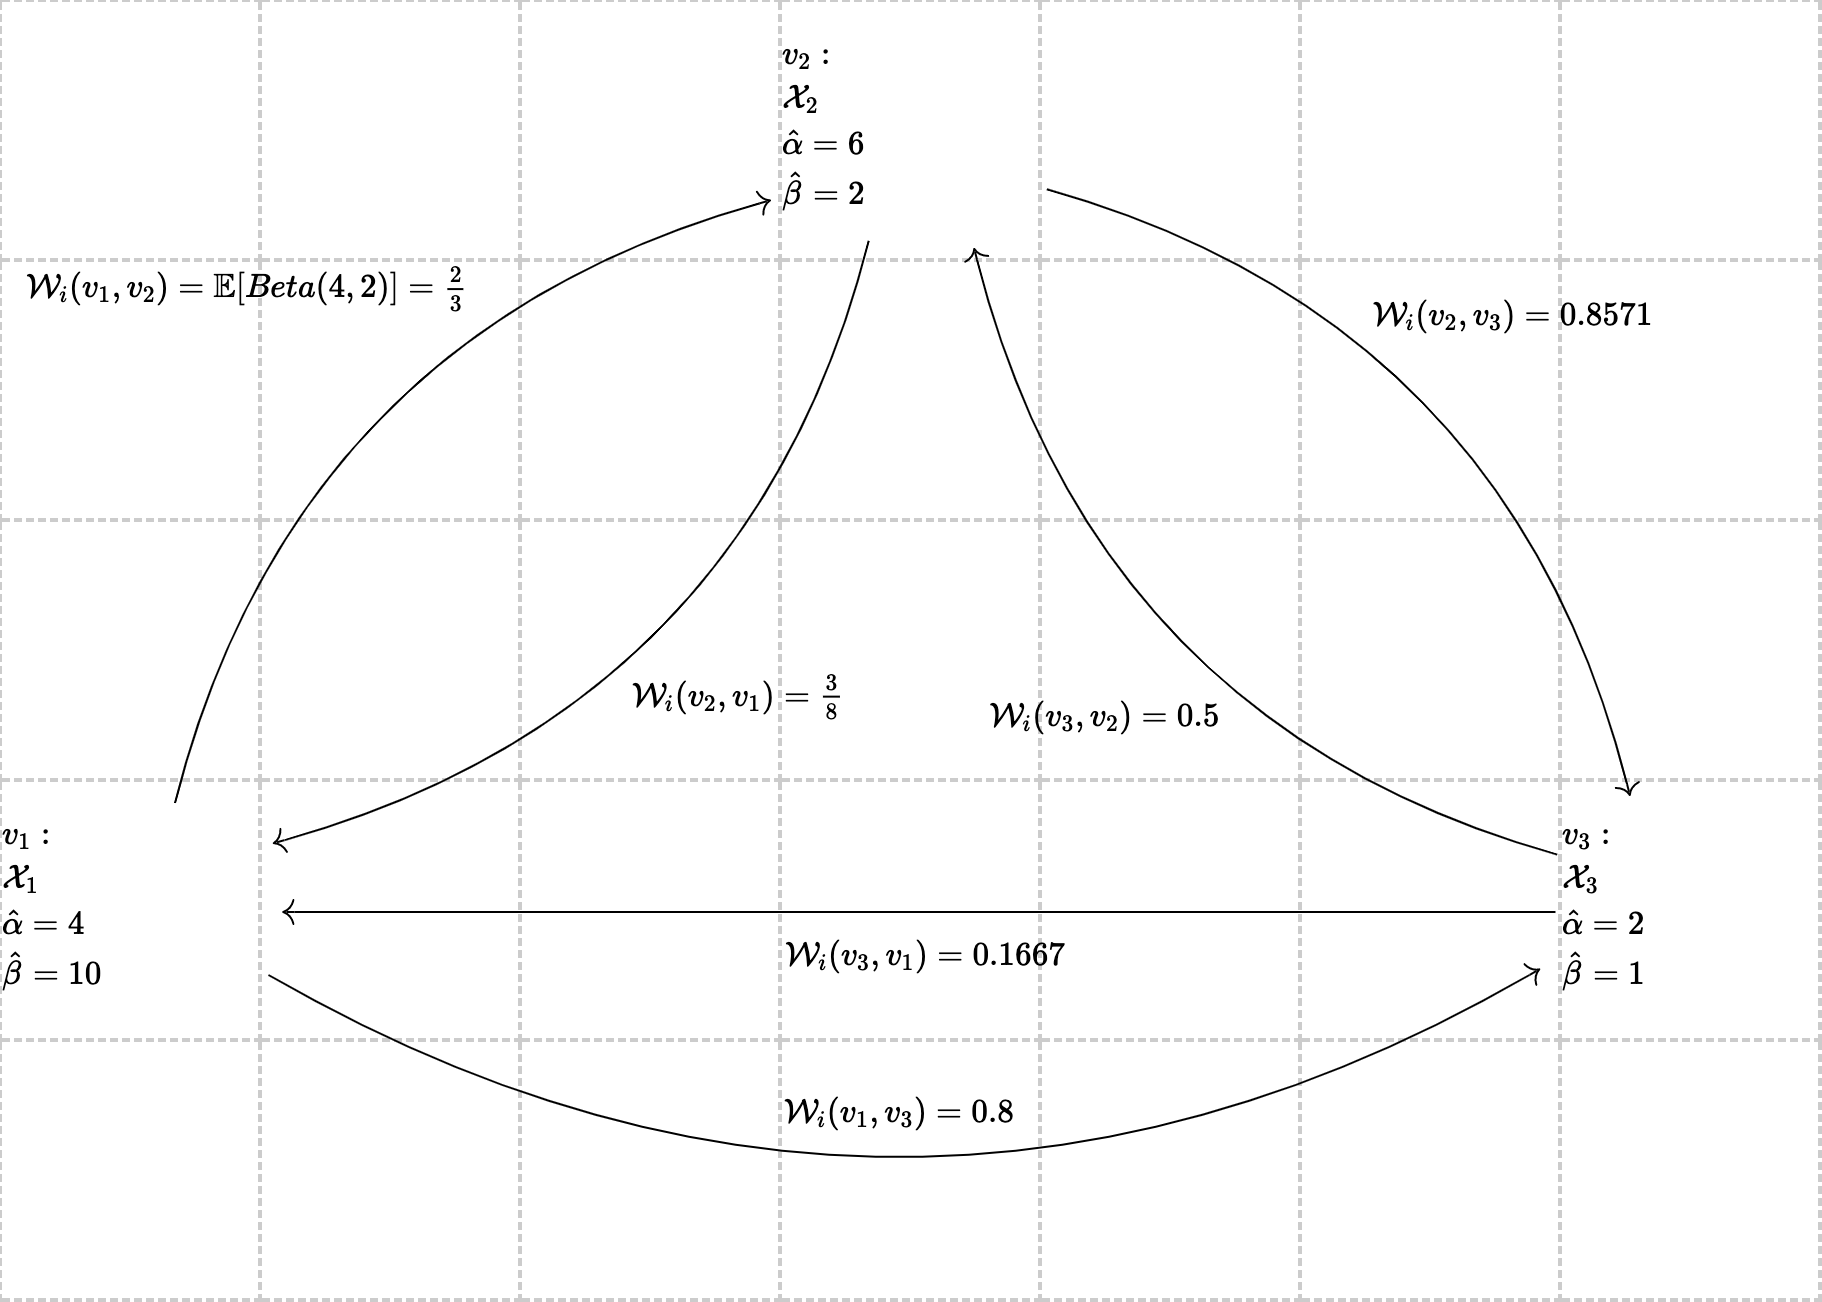
\includegraphics[width=\textwidth]{images/beta_ex.png}
	\caption{An example of a Beta posterior that shows information flowing from $v_1$ to $v_3$.}
	\label{fig:beta-ex}
\end{figure}
There is a wide array of literature on the use of Exponential-families for the modeling of edge weight priors. In particular, the work of Bolla \cite{bolla_estimating_2017} is important. In this work, edge weights are modeled by conditionally independent Beta distributions. The parameters of these Beta distributions are updated via a closed-form solution but it serves as a good model for prediction propogation of information or material from one node to another and converging on a steady-state for the propogation. In the case of GNNs, one can imagine the \verb|MSG| operation as the sending of information. The dense layers in the \verb|Upd| step, then, learn the weight to assign to each incoming and outgoing message. In this vein, the Beta model can approximate this "attention" that is paid in the \verb|Upd| step. Hence, the goal of this model is to serve as an approximiation of this process and encode the steady-state flow of information in the model.
\begin{figure}[t]
	\centering
	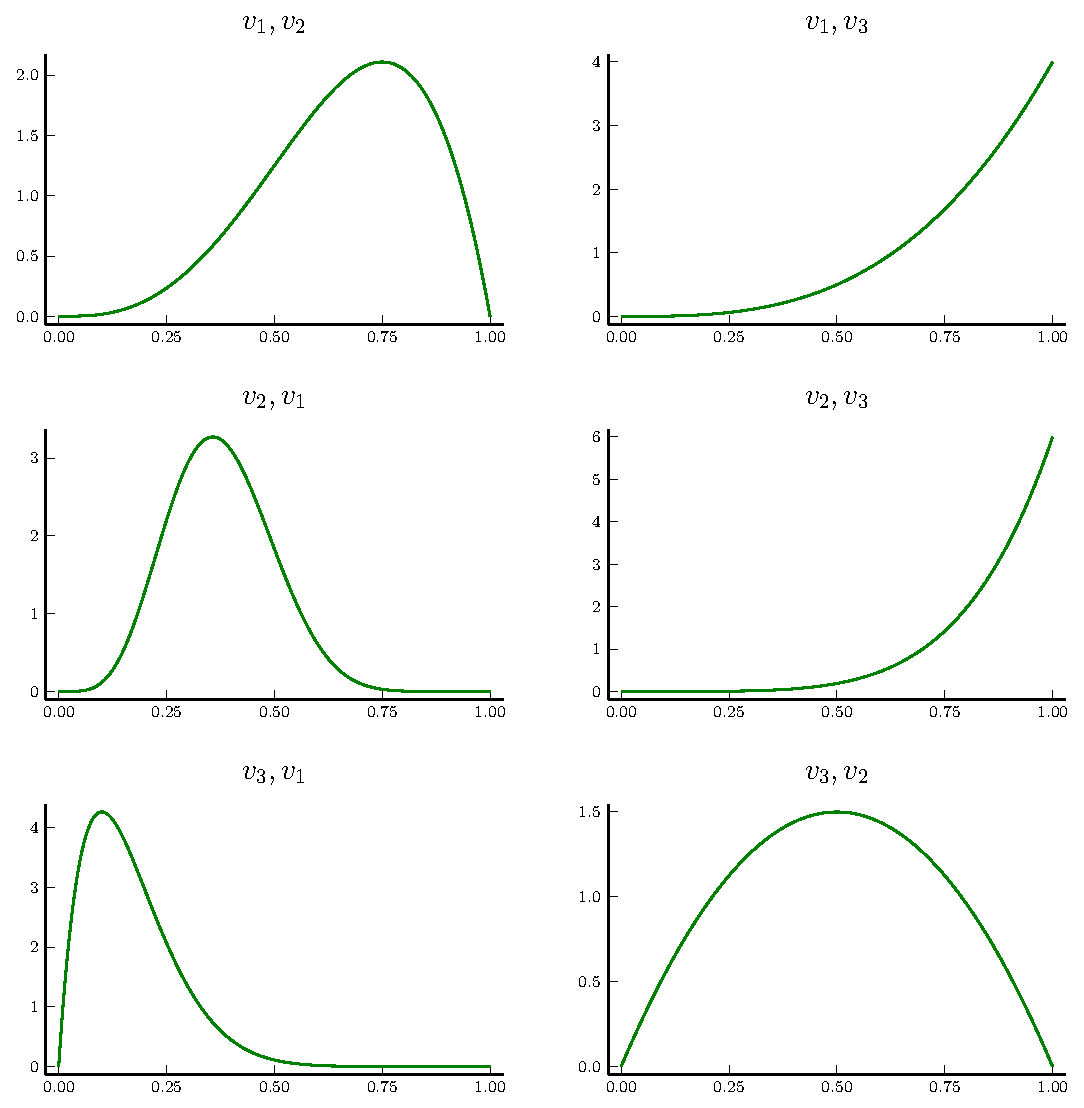
\includegraphics[width=0.8\textwidth]{images/beta_post.pdf}
	\caption{Posterior distributions for each edge in \ref{fig:beta-ex}}
	\label{fig:beta-ex-post}
\end{figure}

In this model, the $\alpha$ values serve to desribe the affinity for information to flow out of a node while the $\beta$ values tend to describe the affinity for information to flow into the node. Together, they describe the steady state flow of information and perfectly describe many networks in which pathways of information lead to end-goal expression. Indeed, since GNNs tend to embed this type of information flow in a deep-learning setting, it serves to reason that such a prior would be a good encapsulation of the process of information flow, especially at steady state. A typical example of this is gene expression in biology \cite{petralia_new_2016} where paths of edges represent regulatory pathways directly. 

An example of this flow can be seen in figure \ref{fig:beta-ex}. In this figure, we consider a hypothetical posterior for this model and demonstrate how it describes the flow of information from node $v_1$ to $v_3$ via these $\alpha$ and $\beta$ parameters. Additionally, in figure \ref{fig:beta-ex-post}, one can see the posterior distribution of each edge. Notably, there is no conditional independence in this model as changing the parameter on one node changes all adjoining edges.

\subsubsection{Training the Beta Model}
While \cite{bolla_estimating_2017} demonstated a novel technique to train the parameters to get the true posterior in the limit, this paper will use a standard SVI setup to train the posterior. In the \verb|Pyro| framework, all SVI runs need two things: the forward model and the variational guide. In listing \ref{alg:beta-model}, both the model is shown and the guide follows a very similar setup since it has the same esxact structure. Note that in both cases the mask is sampled from a beta distribution as defined above. Most GNNs have an effective computational graph size as denoted by the number of layers that are in the model. This effective computational graph is generally, the $l$-hop neighborhood around $v_i$ so we only consider interpretation on $\mathcal{N}_l(v_i, E)$ as the other nodes cannot have any influence. Analogously, let all the nodes in this $l$-hop neighborhood be $V_{i,l}$.
\begin{algorithm}[h]
	\centering
	\caption{The model setup for the Beta model}
	\label{alg:beta-model}
	\begin{algorithmic}
		\Require $v_i \in V, \bar{\alpha} > 0, \bar{\beta} > 0$
		\Require $c \sim \phi(v_i, \mathcal{X}, \mathcal{N}_l(v_i, E), \mathcal{W})$
		\State $\alpha \gets [\bar{\alpha} \mid \forall v_j \in V_{i,l}]$
		\State $\beta \gets [\bar{\beta} \mid \forall v_j \in V_{i, l}]$
		\State $\mathcal{W}_i(v_j, v_k) \sim Beta(\alpha_j, \beta_k) \quad\quad \forall (v_j, v_k) \in \mathcal{N}_l(v_i, E)$
		\State $\hat{y} \gets \phi(v_i, \mathcal{X}, \mathcal{N}_l(v_i, E), \mathcal{W}_i)$
		\State $\hat{c} \sim \hat{y}$
	\end{algorithmic}
\end{algorithm}

The SVI algorithm then optimizes against the $\alpha$ and $\beta$ parameters to match the variational distribution $\hat{y}$ as closely as possible to the full distribution $\phi(v_i, \mathcal{X}, \mathcal{N}_k(v_i, E), \mathcal{W})$. Note that in the case of a graph classification task, the model $\phi$ simply loses its dependence on $v_i$ and we compare against $\phi(\mathcal{X}, E, \mathcal{W})$. They are the exact same formulation. In each epoch of the SVI inference, only one sample is used to get an estimate of the ELBO as is the standard practice \cite{jospin_hands-bayesian_2022}. While this gives a noisy estimate, over time, the value of the ELBO should increase to indicate a better model fit.

\subsection{Normalizing Flow Models}
In this work, there are two specific normalizing flow models that are tested. In one, the system is trained using SVI to utilize the ELBO as the objective, while in the other a simple KL-divergence is computed and the parameters of the normalizing flow are directly optimized using an appropriate SGD algorithm.

\subsubsection{Spline Coupling Normalizing Flows}

\section{Experimental Setup}
\section{Results}
\section{Discussion}

\subsection{Comparison of Models}
Overall, there a few takeaways in comparing the models. The first is that both of the Bayesian models for GNN interpretability perform better than GNNExplainer and represents and increase in the performance of GNN Interpretation methods. While the increase in performance is not too much higher than what GNNExplainer achieves, in a more complicated dataset the difference may be higher.

These Bayesian models not only offer better performance than GNNExplainer, but they also give a deeply introspectable look at the edge interpretations and allow for a detailed analysis of the influnce that the computational graph has on the GNNs performance. The Beta model serves as a low variance estimate for the first mode in the edge mask distribution and is very useful for understanding the high-level pathways of information flow in a GNN. The Normalizing Flow model, though, captures more modalities in the edge mask posterior and is able to give even further details about the GNN. This comes at the expense, though, of a higher variance estimate and more uncertainty in its predictions. 

Together, though, these two models can be very helpful for extracting real-world value out of GNNs. When the computational graph maps to a physical phenomenom, the interpretations from these methods can deliver useful insights that the GNN has learned. GNNExplainer struggles to provide such value and, certainly, cannot capture all the different modalities that the normalizing flow explainer is able to pick up on.

That being said, these models are a lot more computationally expensive with GNNExplainer operating at 10x speed advantage compared to the Bayesian models. While this is quite slow, in reality, one rarely needs to perform analysis on every node on a graph and usually researchers pick notable examples for analysis \cite{bigness_integrating_2021}. Still, this is a significant speed advantage that GNNExplainer holds. 

\subsection{Future Work}
Listed below is a inexhaustive list of various ways in which this research can be taken further. 

\subsubsection{Collation of Examples in Classification Datasets}
One avenue of future work is to combine the ideas of PGExplainer \cite{luo_parameterized_2020} with the Bayesian inference models. Specifically, PGExplainer learns a parametrized network to generate node-level explanations that were trained across all nodes. In this sense, PGExplainer learns more general patterns in the GNN. While learning at each individual neighborhood of each node independently should converge on the same generic truth, leveraging an entire dataset in graph classification or node classification could greatly shorten the amortized inference time that is needed for this model. Especially in the graph embedding experiment, many explanations were similar and creating a parametrized version of the Bayesian inference models could help achieve lower variance estimates at a lower runtime cost.

\subsubsection{Beta Model Conditional Parameter Selection}
The Beta Model is quite restrictive in the set of posteriors that it can learn due to the fixed alpha and beta parameters at each node. While this allows it to achieve low variance estimates for the most important pathways in the GNN, it precludes it from learning the multi-modal distribution that the Normalizing Flow model manages to. Because of this, it may be useful to put a flexible distribution over the alpha and beta values at each node which is conditional on the edge that is being sampled. In this way, the Beta Model could become more flexible while retaining a lot of the nice qualities that it has. 

\subsubsection{Real-World Datasets (SERGIO and Beyond)}
Finally, it would be great to apply these methods to a real-world dataset in order to demonstrate the ability of the full posterior edge mask distribution to capture important information in real-world context. A great usecase comes from computational biology and identifying gene-regulatory networks. In gene-regulatory networks, there are multiple different pathways that all interact in order to regulate gene expression. In a case like this, it would interesting to see what a GNN interpretation framework like the Normalizing Flow model and Beta model would be able to say about these networks. One place to find such a dataset is the SERGIO \cite{dibaeinia_sergio_2020} method that was discussed in \S\ref{sec:sergio}. While a synthetic dataset, it provides this exact type of causal playground upon which interpretation methods can be tested to determine their usefulness as a research tool in biological sciences and beyond.

\newpage


\bibliographystyle{unsrt}
\small{\bibliography{refs}}
\end{document}
